\section{实验二 \quad 存储器与控制器实验(单周期CPU取指译码)}

本次实验开始涉及MIPS架构CPU的设计,其中涵盖CPU在流水线设计中所分割的两个阶段,以下为实验概述:

MIPS架构CPU的传统流程可分为取指、译码、执行、访存、回写(Instruction Fetch, Decode, Execution, Memory Request, Write Back),五阶段。实验一完成了执行阶段的ALU部分,并进行了简单的访存实验,本实验将实现取指、译码两个阶段的功能。

在进行本次实验前,你需要具备以下实验环境及基础能力:
\begin{enumerate}
    \item 了解Xilinx Block Memory Generator IP的使用
    \item 了解数据通路、控制器的概念
\end{enumerate}

\subsection{实验目的}

\begin{enumerate}
    \item 了解随机存取存储器RAM的原理;
    \item 掌握调用Xilinx库IP(Block Memory Generator)实例化RAM的方法;
    \item 掌握单周期CPU各个控制信号的作用和生成过程。
    \item 掌握单周期CPU控制器的工作原理及其设计方法。
    \item 理解单周期CPU执行指令的过程。;
    \item 掌握取指、译码阶段数据通路、控制器的执行过程。
\end{enumerate}
\subsection{实验设备}
\begin{enumerate}
    \item 计算机1台(尽可能达到8G及以上内存);
    \item Nexys4 DDR实验开发板;
    \item Xilinx Vivado开发套件(2019.1版本)。

\end{enumerate}
\newpage
\subsection{实验任务}
\subsubsection{实验要求}
图~\ref{fig:fetch_decode}为本次实验所需完成内容的原理图,依据取指、译码阶段的需求,分别需要实现以下模块:
\begin{figure}[htbp]
    \centering
    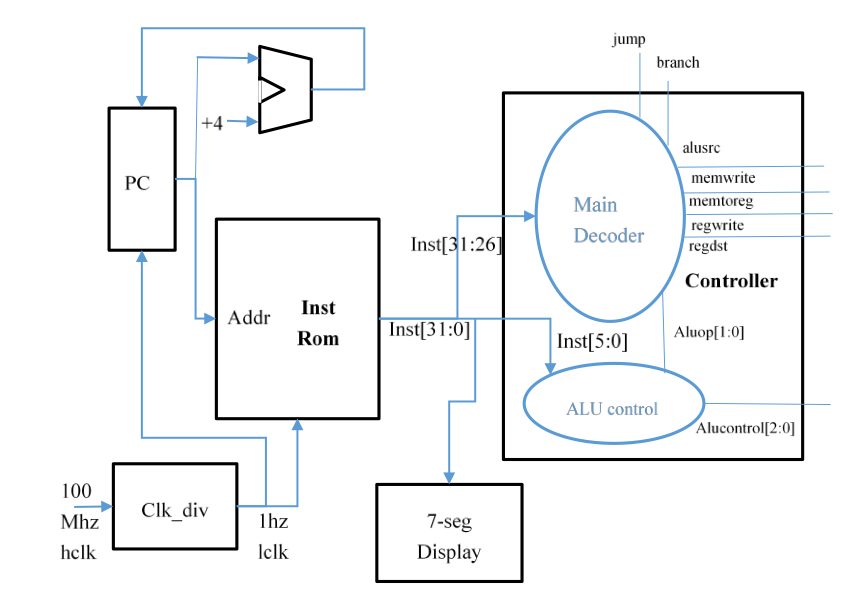
\includegraphics[width = 0.8\textwidth]{image/1_section/fetch_decode.png}
    \caption{取指译码原理图}
    \label{fig:fetch_decode}
\end{figure}

\begin{enumerate}
    \item PC。D触发器结构,用于储存PC(一个周期)。需\textcolor{red}{实现2个输入},分别为\textit{clk, rst},分别连接时钟和复位信号;需\textcolor{red}{实现2个输出},分别为\textit{pc, inst\_ce}, 分别连接指令存储器的\textit{addra, ena}端口。其中\textit{addra}位数依据coe文件中指令数定义;
    \item 加法器。用于计算下一条指令地址,需\textcolor{red}{实现2个输入,1个输出},输入值分别为当前指令地址\textit{PC、32’h4};
    \item Controller。其中包含两部分:
    \begin{enumerate}
        \item main\_decoder。负责判断指令类型,并生成相应的控制信号。需\textcolor{red}{实现1个输入},为指令inst的高6位\textit{op},输出分为2部分,\textcolor{epubblue}{控制信号}有多个,可作为多个输出,也作为一个多位输出,具体参照~\ref{section:section_3}进行设计;\textit{aluop},传输至alu\_decoder,使alu\_decoder配合\textit{inst}低6位\textit{funct},进行ALU模块控制信号的译码。
        \item alu\_decoder。负责ALU模块控制信号的译码。需\textcolor{red}{实现2个输入,1个输出},输入分别为\textit{funct, aluop};输出位\textit{alucontrol}信号。
        \item 除上述两个组件,需设计controller文件调用两个decoder,\textcolor{epubblue}{对应实现\textit{op,funct}输入信号,并传入调用模块;对应实现控制信号及\textit{alucontrol},并连接至调用模块相应端口}。
    \end{enumerate}

    \item 指令存储器。使用Block Memory Generator IP构造。(参考~\ref{section:section_2})
    
    \textcolor{red}{ 注意:	Basic中Generate address interface with 32 bits 选项不选中;PortA Options中 Enable Port Type 选择为 Use ENA Pin}
    
    \textcolor{gray}{
    \item 时钟分频器。将板载100Mhz频率降低为1hz,连接PC、指令存储器时钟信号clk。(参考数字逻辑实验)\\
    注意:Xilinx Clocking Wizard IP可分的最低频率为4.687Mhz,因而只能使用自实现分频模块进行分频
    }
\end{enumerate}


\subsubsection{实验步骤}

\begin{enumerate}
    % \item 从实验一、数字逻辑课程实验中,导入Display、clk\_div模块
    \item 创建PC模块
    \item 创建main\_decde, alu\_decode模块
    \item 创建Controller,调用main\_decode, alu\_decode
    \item 使用Block Memory,导入coe文件
    \item 自定义顶层文件,连接相关模块
    \item \textbf{自行编写Testbench仿真文件,时钟周期设为10ns,每个时钟周期输入地址Address + 4,捕获输出信号并打印在控制台。}\\
        \textcolor{red}{打印格式:instruction: 32'h00000000, memtoreg: 1, memwrite: 0, .....}
\end{enumerate}

\textcolor{gray}{
Controller输出信号与led管脚对应关系如下表:
}
\begin{table}[htbp]
    \centering
    \color{gray}
    \begin{tabular}{c|c|c|c|c|c|c|c|c}
         memtoreg&	memwrite&	pcsrc&	alusrc&	regdst&	regwrite&	jump&	branch&	alucontrol  \\ \hline
         [0:0]&	[0:0]&	[0:0]&	[0:0]&	[0:0]&	[0:0]&	[0:0]&	[0:0]&	[2:0] \\ \hline
         led[0]&	led[1]&	led[2]&	led[3]&	led[4]&	led[5]&	led[6]&	led[7]&	led[8:10] \\ \hline
    \end{tabular}
    \caption{\textcolor{gray}{输出信号与led管脚}}
    \label{tab:controller_sig}
\end{table}

% 本次实验使用Vivado的Block Memory Generator模拟数据在存储器中的存取过程。实验使用单端口ROM。初始化ROM存储器中的内容,通过开关选择相应的地址,将对应的存储器中内容读出来,并通过七段数码管显示。实验原理如图~\ref{fig:memory_experiment}所示:

% \begin{figure}[htbp]
%     \centering
%     \includegraphics[width = \textwidth]{image/1_section/memory_experiment.png}
%     \caption{Caption}
%     \label{fig:memory_experiment}
% \end{figure}

% \textbf{实验要求:}


\subsection{实验环境}
以下表格中红色部分需自行实现,黑色部分于实验发布包中提供。

\begin{table}[htbp]
    \centering
    \begin{tabu}{|l|l|}
        \hline
        \textcolor{red}{|--top.v}& 设计顶层文件,参照图~\ref{fig:fetch_decode}将各模块连接。 \\
        % \textcolor{red}{|----clk\_div.v} & \textcolor{red}{时钟分频模块,需讲将100MHz的时钟频率降低至1Hz。} \\
        \textcolor{red}{|----pc.v} &\textcolor{red}{D触发器结构。输入为下一条指令地址,输出为当前指令地址。}  \\
        |----ram.ip&RAM IP,通过Block memory generator进行实例化。  \\
        \textcolor{red}{|----controller.v} &\textcolor{red}{ 控制器模块,本次实验重点。} \\
        \textcolor{red}{|------maindec.v} & \textcolor{red}{Main decoder模块,负责译码得到各个组件的控制信号。} \\
        \textcolor{red}{|------aludec.v} & \textcolor{red}{ALU Decoder模块,负责译码得到ALU控制信号。}\\
        \rowfont{\color{gray}}
        |----display.v& 七段数码管显示模块文件,已提供。 \\
        \rowfont{\color{gray}}
        |------seg7.v& 七段数码管显示模块组成文件,已提供。 \\
        \rowfont{\color{gray}}
        |--constr.xdc&综合实现时,约束文件,已提供。  \\
        
        
        \hline
    \end{tabu}
    \caption{实验文件树}
    \label{tab:file_tree}
\end{table}

